\documentclass[english,14pt]{beamer}
\usetheme{EastLansing}
\usecolortheme{spruce}

\usepackage{xcolor}
\usepackage{listings}
\usepackage{courier}
\usepackage{graphicx}
\usepackage{amsmath}
\usepackage{algorithm2e}
\usepackage{multicol}
\usepackage{hyperref}

% http://mirrors.ibiblio.org/CTAN/macros/latex/contrib/datetime2/datetime2.pdf
\usepackage{babel}
\usepackage[useregional]{datetime2}

% https://tex.stackexchange.com/questions/42619/x-mark-to-match-checkmark
\usepackage{pifont}% http://ctan.org/pkg/pifont

%% https://stackoverflow.com/questions/1435837/how-to-remove-footers-of-latex-beamer-templates
%%gets rid of bottom navigation bars
%\setbeamertemplate{footline}[page number]
%
%gets rid of navigation symbols
\setbeamertemplate{navigation symbols}{}


\usefonttheme[onlymath]{serif}

\definecolor{mGreen}{rgb}{0,0.6,0}
\definecolor{mGray}{rgb}{0.5,0.5,0.5}
\definecolor{mPurple}{rgb}{0.8,0,0.82}
\definecolor{backgroundColour}{rgb}{0.95,0.95,0.92}
\definecolor{lightBlue}{rgb}{0.1, 0.1, 0.8}

\newcommand\red[1]{{\color{red} #1}}
\newcommand\green[1]{{\color{green} #1}}
\newcommand\blue[1]{{\color{blue} #1}}

\newcommand{\cmark}{\ding{51}}%
\newcommand{\xmark}{\ding{55}}%

\lstdefinestyle{CStyle}{
    backgroundcolor=\color{backgroundColour},   
    commentstyle=\color{mGreen},
    keywordstyle=\color{magenta},
    numberstyle=\tiny\color{mGray},
    stringstyle=\color{mPurple},
    basicstyle=\footnotesize,
    breakatwhitespace=false,         
    breaklines=true,                 
    captionpos=b,                    
    keepspaces=true,                 
    numbers=left,                    
    numbersep=5pt,                  
    showspaces=false,                
    showstringspaces=false,
    showtabs=false,                  
    tabsize=2,
    language=C
}

\lstdefinestyle{pseudo}{
        basicstyle=\ttfamily\footnotesize,
        keywordstyle=\color{lightBlue},
        morekeywords={BEGIN,END,IF,ELSE,ENDIF,ELSEIF,PRINT,WHILE,RETURN,ENDWHILE,DO,FOR,TO,IN,ENDFOR,BREAK,INPUT},
        morecomment=[l]{//},
        commentstyle=\color{mGreen}
}

\lstset{basicstyle=\footnotesize\ttfamily,breaklines=true}
\lstset{framextopmargin=50pt,tabsize=2}

\title{ENGG1003 - Monday Week 8}
\subtitle{Solving nonlinear algebraic equations }%\\ \& computing integrals}
\author{Steve Weller}
\institute{University of Newcastle}
%\date{\today}
\date{26 April 2021}

% following is a bit of a hack, but forces page numbers (technically: frame numbers) to run 1,2,3,... 
% with titlepage counting as frame 1

\addtocounter{framenumber}{1}
\titlepage

\begin{document}

\begin{flushleft}
{\scriptsize Last compiled:~\DTMnow}
\vspace*{-5mm}
\end{flushleft}
\framebreak

%==============================================================

\begin{frame}[fragile]

\frametitle{Lecture overview}
\begin{enumerate}
	\item Solving nonlinear algebraic equations \red{pp.~175-176}
	\begin{itemize}
		\item generic
		\item two problems: flight time, fluid level
	\end{itemize}
	
	\item[]
	
	\item Bisection method \red{\S7.7}
	
	\item[]
	
	\item Secant method \red{\S7.3}
	\begin{itemize}
		\item Newton--Raphson method
	\end{itemize}
	
	\item[]
	
	\item Extensions
	\begin{itemize}
		\item bisection vs.~secant re-write as functions
		\item timing code in Python
		\item initialisation \& speed comparisons
		\item failure to converge
	\end{itemize}
	
\end{enumerate}

\end{frame}

%==============================================================

\begin{frame}[fragile]

\frametitle{$1)$ Solving nonlinear algebraic equations}

\begin{itemize}
	\item find $x$ satisfying $f(x) = 0$
	\item aka root-finding
\end{itemize}

\end{frame}

%==============================================================

\begin{frame}[fragile]

\frametitle{Flight time}

\begin{itemize}
	\item one more time!
\end{itemize}

\end{frame}

%==============================================================

\begin{frame}[fragile]

\frametitle{Fluid level}

image of measuring cup

\begin{figure}[ht]
	\centering
	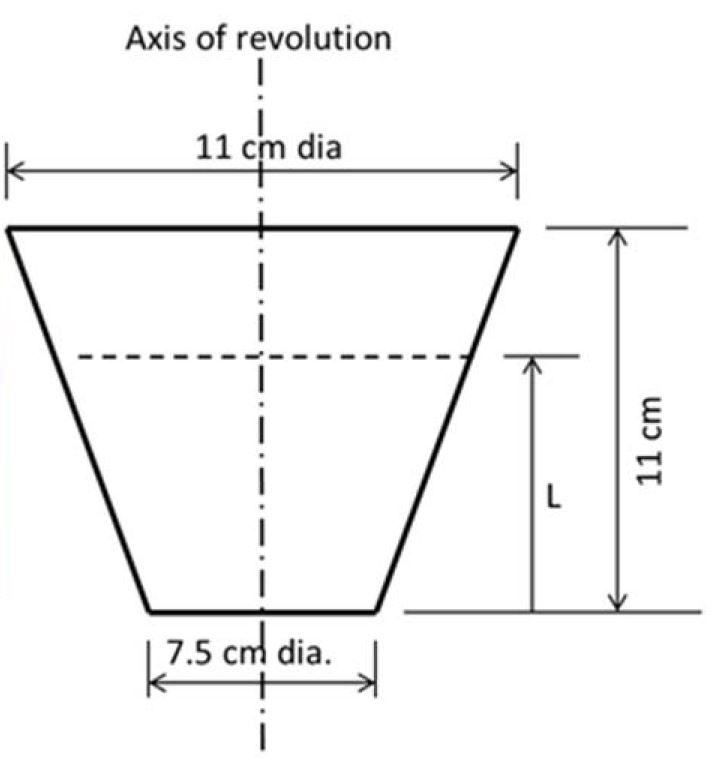
\includegraphics[width=0.5\textwidth]{figures/cupDimensions}
\end{figure}

\end{frame}

%==============================================================

\begin{frame}[fragile]

\frametitle{Fluid level}

% https://www.sjsu.edu/me/docs/hsu-Chapter%2010%20Numerical%20solution%20methods.pdf
% Section 10.3.2

\begin{itemize}
	\item cup dimension figure
	\item water in dam, coal in stockpile
	\item volume $V$ (mL) depends on depth $L$ as follows, \emph{presented without proof:}
	\[
		V = 0.0268L^3 + 1.884L^2 + 44.15L
	\]
	\item Question: depth $L$ when cup holds $500$~mL of water?
	\item solve $f(L) = 0$ where
	\[
		F(L) = 0.0268L^3 + 1.884L^2 + 44.15L - 500
	\]
\end{itemize}

\end{frame}

%==============================================================

\begin{frame}[fragile]

\frametitle{$2)$ Bisection method}

\begin{itemize}
	\item basic idea: visualisation
\end{itemize}

\end{frame}

%==============================================================

\begin{frame}[fragile]

\frametitle{}

\begin{itemize}
	\item bisection method: key equations
\end{itemize}

\end{frame}

%==============================================================

\begin{frame}[fragile]

\frametitle{}

\begin{itemize}
	\item bisection method: pseudocode
\end{itemize}

\end{frame}

%==============================================================

\begin{frame}[fragile]

\frametitle{}

\begin{itemize}
	\item bisection method: Python code
\end{itemize}

\end{frame}

%==============================================================

\begin{frame}[fragile]

\frametitle{}

\begin{itemize}
	\item bisection method: simulation results
\end{itemize}

\end{frame}

%==============================================================

\begin{frame}[fragile]

\frametitle{$3)$ Secant method}

\begin{itemize}
	\item basic idea: visualisation
\end{itemize}

\end{frame}

%==============================================================

\begin{frame}[fragile]

\frametitle{}

\begin{itemize}
	\item secant method: key equations
\end{itemize}

\end{frame}

%==============================================================

\begin{frame}[fragile]

\frametitle{}

\begin{itemize}
	\item secant method: pseudocode
\end{itemize}

\end{frame}

%==============================================================

\begin{frame}[fragile]

\frametitle{}

\begin{itemize}
	\item secant method: Python code
\end{itemize}

\end{frame}

%==============================================================

\begin{frame}[fragile]

\frametitle{}

\begin{itemize}
	\item secant method: simulation results
\end{itemize}

\end{frame}

%==============================================================

\begin{frame}[fragile]

\frametitle{}

\begin{itemize}
	\item xxx
\end{itemize}

\end{frame}

%==============================================================

\begin{frame}[fragile]

\frametitle{$4)$ Computing integrals}

\begin{itemize}
	\item xxx
\end{itemize}

\end{frame}

%==============================================================

\begin{frame}[fragile]

\frametitle{}

\begin{itemize}
	\item xxx
\end{itemize}

\end{frame}

%==============================================================

\begin{frame}[fragile]

\frametitle{Lecture summary}
\begin{itemize}
	\item Solving nonlinear algebraic equations

	\item[]
	
	\item Bisection method

	\item[]
	
	\item Secant method
	\begin{itemize}
		\item Newton--Raphson method
	\end{itemize}

	\item[]
	
	\item Extensions
	
\end{itemize}

\end{frame}

\end{document}